\section{Results}
\label{sec:dihiggs_result}
%-------------------------------------------------------------------------------

The data yields in all signal regions are currently blinded. In order to quantify the sensitivity of the expected background and signal, cross section $\sigma_{H}$ limits on $pp \to hh$ production are set as a function of  $m_{hh}$ in the range 500 GeV to 3000 GeV and for the non-resonant signal. A simultaneous maximum-likelihood fit is performed for the number of events in the signal region and three control regions. Two of these correspond to the $\text{m}_{bb}$ sideband region as defined in Section~\ref{subsec:topCR}, with one A region and one C region as described in Section~\ref{sec:multijet}. The third control region corresponds to the signal region using the C region selection criteria.

The fit includes six contributions: signal, $W$+jets, $Z$+jets, $t\bar{t}$, single-top, diboson and multi-jet. The $t\bar{t}$ and multi-jet normalizations factors are free to float in the global fit while the diboson, $W$+jets and $Z$+jets backgrounds are constrained to their expected Standard Model cross-section within uncertainties. The $t\bar{t}$ modeling systematic uncertainties are applied to the yields in the signal region only as they have been extrapolated from the top control region, as described in Section~\ref{sec:topsys}.

The event numbers in the different regions are then modeled as:
\begin{align*}
&N_\text{SR,A} = \sigma_\text{sig}\mu N^\text{SR,A}_\text{sig} + \sigma_{t\bar{t}}\mu_{t\bar{t}}N^\text{SR,A}_{t\bar{t}} + \sigma_\text{QCD}\mu_\text{QCD}N^\text{SR,A}_\text{QCD} + \sigma_\text{BG}N^\text{SR,A}_\text{BG} \\
&N_\text{SR,C} = \sigma_\text{sig}\mu N^\text{SR,C}_\text{sig} + \mu_{t\bar{t}}N^\text{SR,C}_{t\bar{t}} + \frac{1}{R}\left(\frac{N_\text{D}}{N_\text{B}}\right)\sigma_\text{QCD}\mu_\text{QCD}N^\text{SR,A}_\text{QCD} + \sigma_\text{BG}N^\text{SR,C}_\text{BG} \\
%&N_\text{SR,C} = c \cdot\sigma_\text{sig}\mu N^\text{SR,C}_\text{sig} + \mu_{t\bar{t}}N^\text{SR,C}_{t\bar{t}} + \frac{1}{R}\left(\frac{N_\text{D}}{N_\text{B}}\right)\sigma_\text{QCD}\mu_\text{QCD}N^\text{SR,A}_\text{QCD} + \sigma_\text{BG}N^\text{SR,C}_\text{BG} \\
&N_{\text{m}_{bb},\text{A}} = \sigma_\text{sig}\mu N^{\text{m}_{bb},\text{A}}_\text{sig} + \mu_{t\bar{t}}N^{\text{m}_{bb},\text{A}}_{t\bar{t}} + \sigma_\text{QCD}\mu_\text{QCD}N^{\text{m}_{bb},\text{A}}_\text{QCD} + \sigma_\text{BG}N^{\text{m}_{bb},\text{A}}_\text{BG} \\
&N_{\text{m}_{bb},\text{C}} = \sigma_\text{sig}\mu N^{\text{m}_{bb},\text{C}}_\text{sig} + \mu_{t\bar{t}}N^{\text{m}_{bb},\text{C}}_{t\bar{t}} + \frac{1}{R}\left(\frac{N_\text{D}}{N_\text{B}}\right)\sigma_\text{QCD}\mu_\text{QCD}N^{\text{m}_{bb},\text{A}}_\text{QCD} + \sigma_\text{BG}N^{\text{m}_{bb},\text{C}}_\text{BG} \\
%&N_{\text{m}_{bb},\text{C}} = c \cdot \sigma_\text{sig}\mu N^{\text{m}_{bb},\text{C}}_\text{sig} + \mu_{t\bar{t}}N^{\text{m}_{bb},\text{C}}_{t\bar{t}} + \frac{1}{R}\left(\frac{N_\text{D}}{N_\text{B}}\right)\sigma_\text{QCD}\mu_\text{QCD}N^{\text{m}_{bb},\text{A}}_\text{QCD} + \sigma_\text{BG}N^{\text{m}_{bb},\text{C}}_\text{BG} \\
\end{align*}
%\textbf{we need a further equation for the C region of Top CR, and two
%$\mu_{\rm QCD}$ one to estimate QCD in SR and a second to estimate QCD in SR}
where $\mu$ is the signal strength of the $hh\rightarrow bbWW$ production %, 
%$c = N_\text{SR,C}^\text{sig}/N_\text{SR,A}^\text{sig}$ is the signal leakage into 
%control region C of the multi-jet estimate 
and $(RN_\text{B}/N_\text{D})^{-1}$ is the
fraction of multi-jet events in the signal region that appear in region C.
The $\sigma_i$ represent the systematic uncertainties associated to each contribution.


%The signal leakage, $c$, and the fraction of multi-jet events from the signal region in
%region C, $(RN_\text{B}/N_\text{D})^{-1}$, are taken as external inputs to the fit. 
%The signal leakages for each selection and signal sample are presented in Table~\ref{tab:leakages}.
%\begin{table}[t]
%\centering
%\begin{tabular}{rccccc}\hline\hline
%\multicolumn{6}{c}{Non-resonant selection}\\
%Signal leakage  &  0.11 $\pm$ 0.04 & & & & \\ \hline \hline
%\multicolumn{6}{c}{Low-mass selection}\\
%$m_H$ (GeV) & 500 & 600 & 700 & 750 & 800 \\
%Signal Leakage & 0.04 $\pm$ 0.02 & 0.08 $\pm$ 0.02 & 0.07 $\pm$ 0.02 & 0.10 $\pm$ 0.02 & 0.09 $\pm$ 0.02 \\ \hline
%$m_H$ (GeV) & 900 & 1000 & 1100 & 1200 & 1300 \\
%Signal Leakage &0.09 $\pm$ 0.02 & 0.05 $\pm$ 0.01 & 0.08 $\pm$ 0.02 & 0.10  $\pm$ 0.02 & 0.06 $\pm$ 0.01 \\ \hline\hline
%\multicolumn{6}{c}{High-mass selection}\\
%$m_H$ (GeV) & 1300 & 1400 & 1500 & 1600 & 1800 \\ 
%Signal Leakage & 0.063 $\pm$ 0.007 & 0.068 $\pm$ 0.007 & 0.052 $\pm$ 0.007 & 0.053 $\pm$ 0.007 & 0.07 $\pm$ 0.02 \\ \hline
%$m_H$ (GeV) & 2000 & 2250 & 2500 & 2750 & 3000 \\ 
%Signal Leakage & 0.08 $\pm$ 0.01 & 0.11 $\pm$ 0.03 & 0.04 $\pm$ 0.01 & 0.06 $\pm$ 0.02 & 0.04 $\pm$ 0.02  \\
%\hline\hline
%\end{tabular}
%\caption{Fraction of signal events in the signal region in multi-jet control region C after all selection criteria for all selections.}\label{tab:leakages}
%\end{table}

The factor $(RN_\text{B}/N_\text{D})^{-1}$ is obtained as described in Section~\ref{sec:multijet}. The initial values of the $t\bar{t}$ normalization factor and number of multi-jet events in the signal region are extracted from the third iteration of the stability test.%

%Limits on resonant $hh\rightarrow bbWW$ production cross section are set by performing
%counting experiments over relevant ranges of $m_{hh}$, defined such that the event
%selection efficiency is 75\% for each signal sample. 
%The production di-Higgs resonances of masses ranging from 500~GeV to 3000~GeV is studied.

The fit is performed combining electron and muon channels into a single data yield. Systematic uncertainties are taken into account as nuisance parameters with Gaussian sampling distributions. For each source of systematic uncertainty, the correlations across bins and between different kinematic regions as well as those between signal and background are taken into account. The statistical analysis of the final results are based on the statistical framework used in previous Run 1 higgs~~\cite{Aad:2012an} and dihiggs~~\cite{Aad:2052848} analyses. Fitting and input models are handled by the RooStats~~\cite{2010acat.confE..57M} and RooFit~~\cite{2003physics...6116V} packages. Complete information about the statistical treatment and asymptotic formulae used to calculate the limits can be found elsewhere~\cite{Cowan:2010js}. Profile-likelihood-ratio test statistics are used to 
%measure the compatibility of the background-only
%hypothesis with the observed data and to 
test the hypothesis of Higgs boson pair production with its cross section as the parameter of interest. The likelihood is the product of terms of the Poisson probability constructed from the final discriminant and of nuisance parameter constraints with either Gaussian, log-normal, or Poisson distributions. Upper limits on the Higgs boson pair production cross section are derived using the CL$_\text{s}$ method~\cite{0954-3899-28-10-313}.

The expected upper limit at 95\% CL on the cross-section for non-resonant Higgs boson pair production times branching fraction $\sigma(pp \to hh) \cdot {\rm Br(hh}\to\rm{ \bbWW})$ is $1.58\left(^{+0.62}_{-0.44}\right)$~pb  which is equivalent to 191 times the SM prediction of 0.03341~pb.

The expected and observed upper limits at 95\% CL on the cross-section of resonant production as a function of mass is shown in Figure~\ref{fig:finalLimit}. The low-mass selection is used for resonances of mass up to 1600~GeV. The high-mass selection is used for resonances of mass 1800~GeV and above. The most stringent observed (expected) limit is found for a resonant mass of 2500 GeV at 0.23 (0.45) pb. The largest deviation between the observed and expected limits is found at a resonance mass of 1800 GeV and has a local significance of 1.87 $\sigma$. The distribution of the standard deviation of observed limits with respect to the expected limits ( (observed limit - expected limit) / one sigma expected deviation) is shown in Figure~\ref{fig:limitSigmaDistribution}. The red line shows a Gaussian fit with a mean of zero and a sigma of one and has a $\chi^2/$ndf of $2.86/3$. This is consistent with an overall observation of zero signal.

%All the upper cross-section limits presented in this section include MC statistical uncertainties and $t\bar{t}$ modelling systematic uncertainties only.

Figures~\ref{fig:pullPlots1_mu_uncond} and ~\ref{fig:pullPlots2_mu_uncond} show pull and ranking plots for all systematics included as nuisance parameters in the fit. Plots for m$_X$ = 700, 900, 2250, and 3000 GeV for are shown using Asimov datasets\footnote{An Asimov dataset is an artificial, generated dataset where all simulation inputs are set to their expected values~\cite{Cowan:2010js}.} profiled with the signal strength parameter set to zero. The 700 and 900 GeV mass points are evaluated using the low-mass selection while the 2250 and 3000 GeV points are evaluated using the high-mass selection. %The pulls and rankings look reasonable for all presented masses.

The analysis presented in this chapter represents the first ever attempt to measure dihiggs production in the semileptonic \bbWW final state. Several updates and changes have been made between the version of the analysis presented in this dissertation and the final version published by the ATLAS collaboration. The published version uses a cutflow that was re-optimized by taking into account the systematic as well as statistical uncertainties, and the error on the QCD estimation was significantly reduced. These and other improvements lead to overall more sensitive upper limits in the public result, however both the public analysis and the version presented in this dissertation were unblinded together, and the version presented here is internally self-consistent.
\begin{figure}[hb]
\begin{center}
  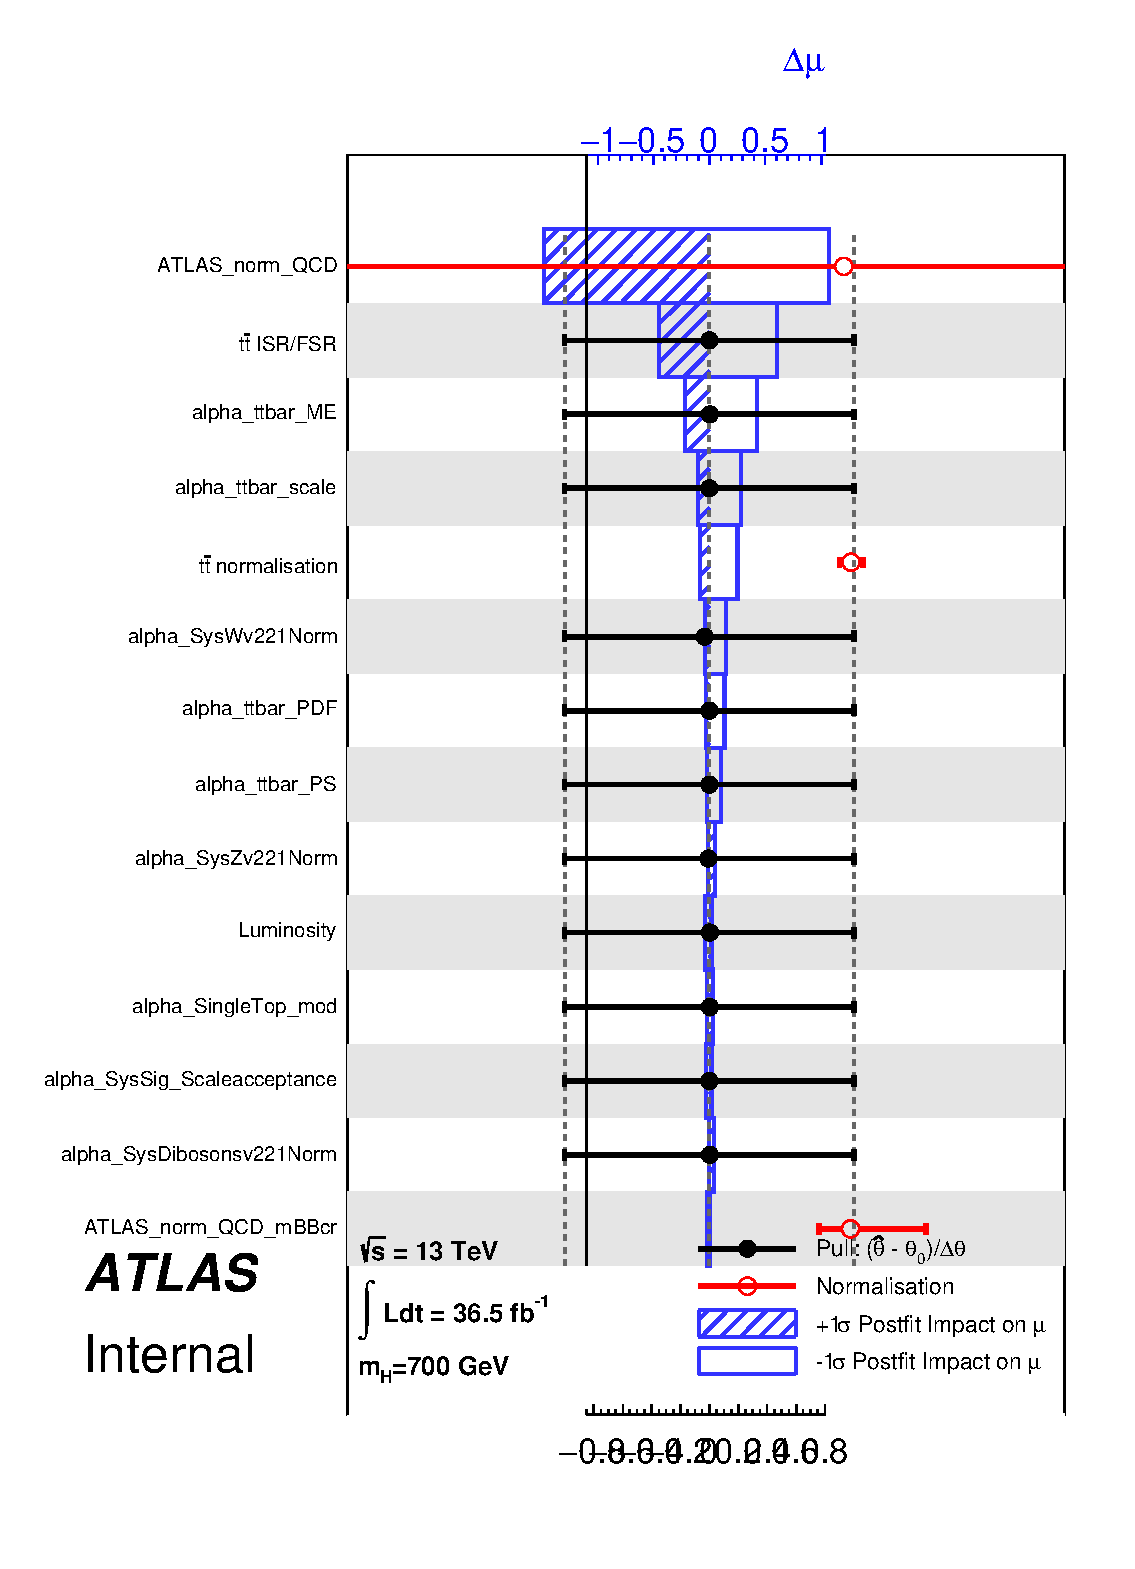
\includegraphics[width=0.45\textwidth]{chapters/dihiggs2/figures/statFit/pullPlot_X700_mu0_unconditional.eps} 
  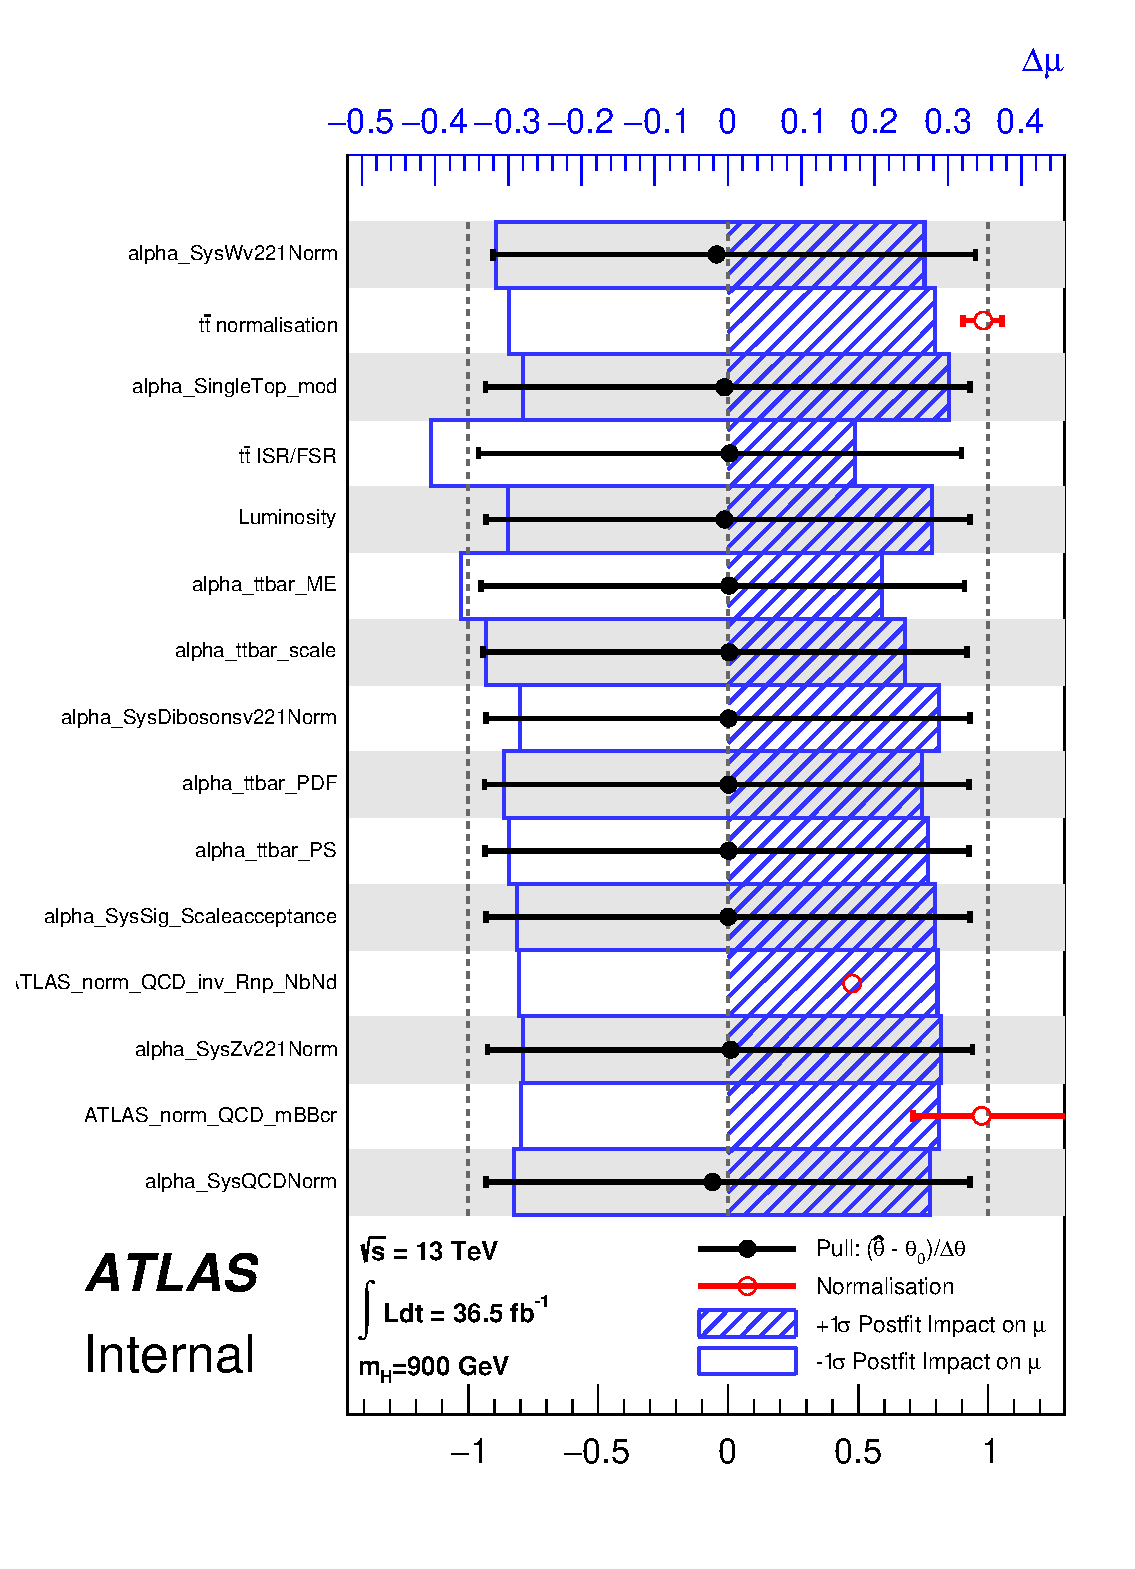
\includegraphics[width=0.45\textwidth]{chapters/dihiggs2/figures/statFit/pullPlot_X900_mu0_unconditional.eps}
   \caption{Pull plots produced when fitting to an Asimov dataset created and profiled at $\mu=0$ for m$_X$ = 700 and 900~GeV for the low-mass selection. The signal strength, $\mu$, is allowed to float as a free parameter during the fit.}
  \label{fig:pullPlots1_mu_uncond}
\end{center}    
\end{figure}
\begin{figure}[hb]
\begin{center}
  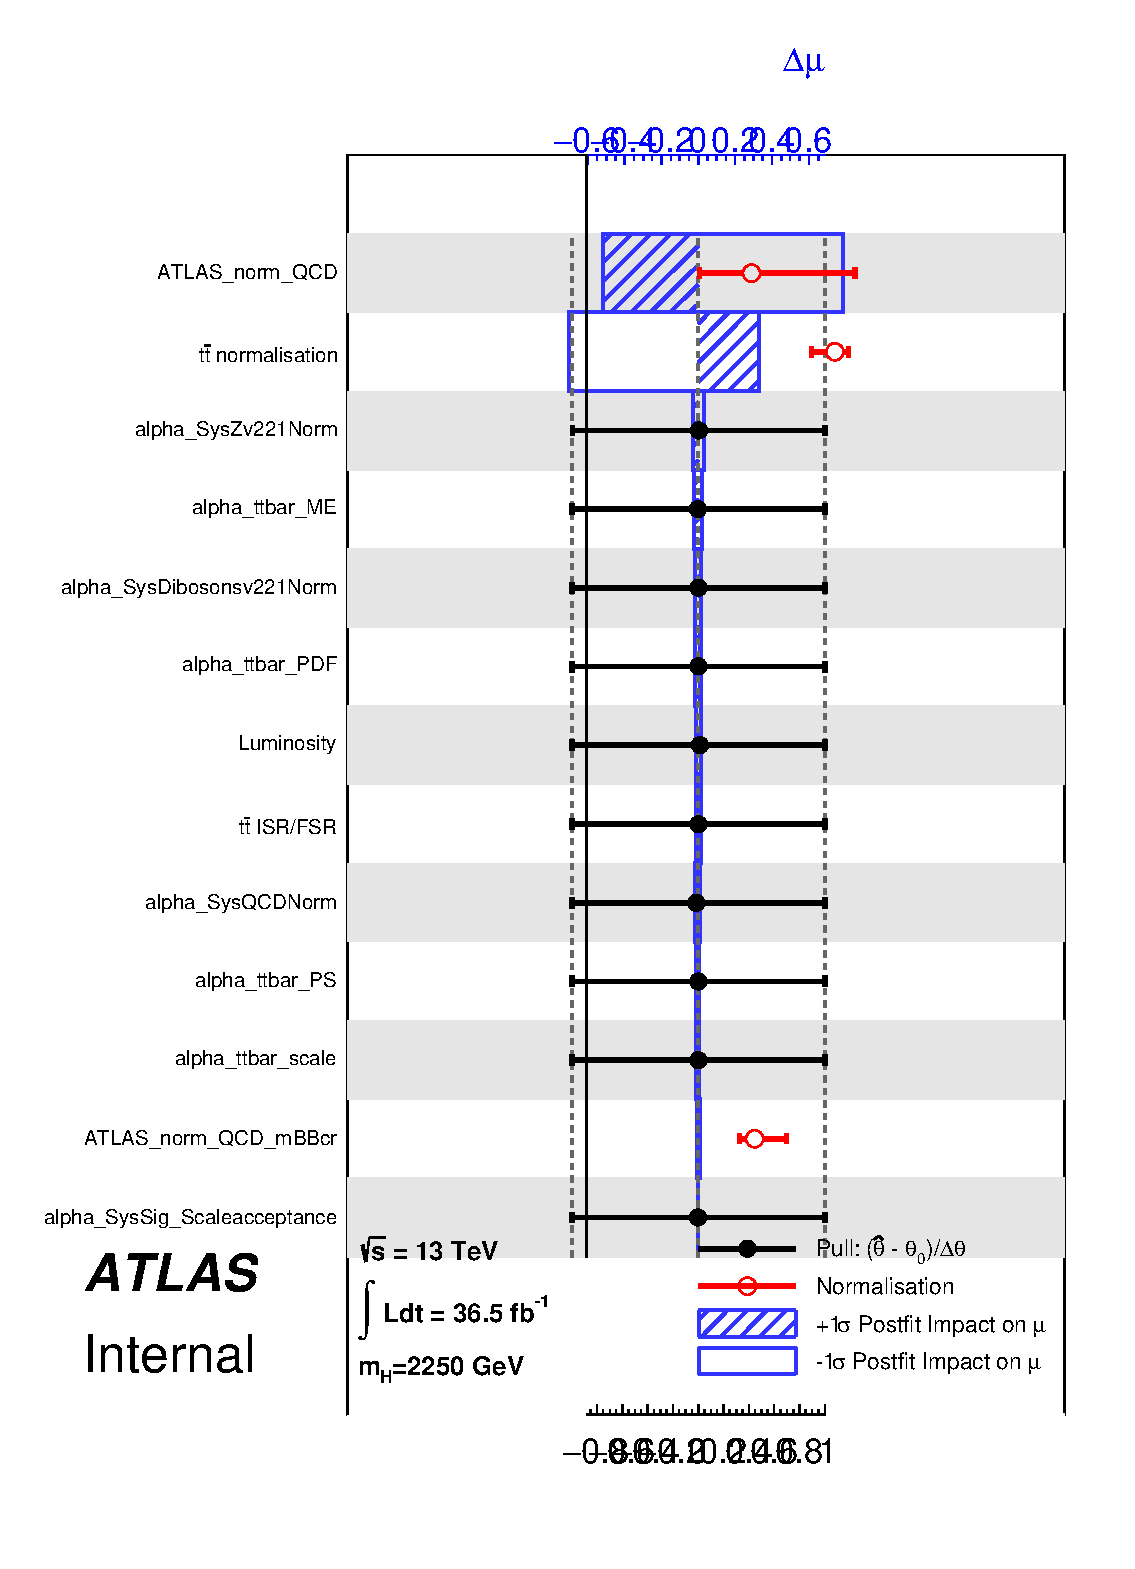
\includegraphics[width=0.45\textwidth]{chapters/dihiggs2/figures/statFit/pullPlot_X2250_mu0_unconditional.eps} 
  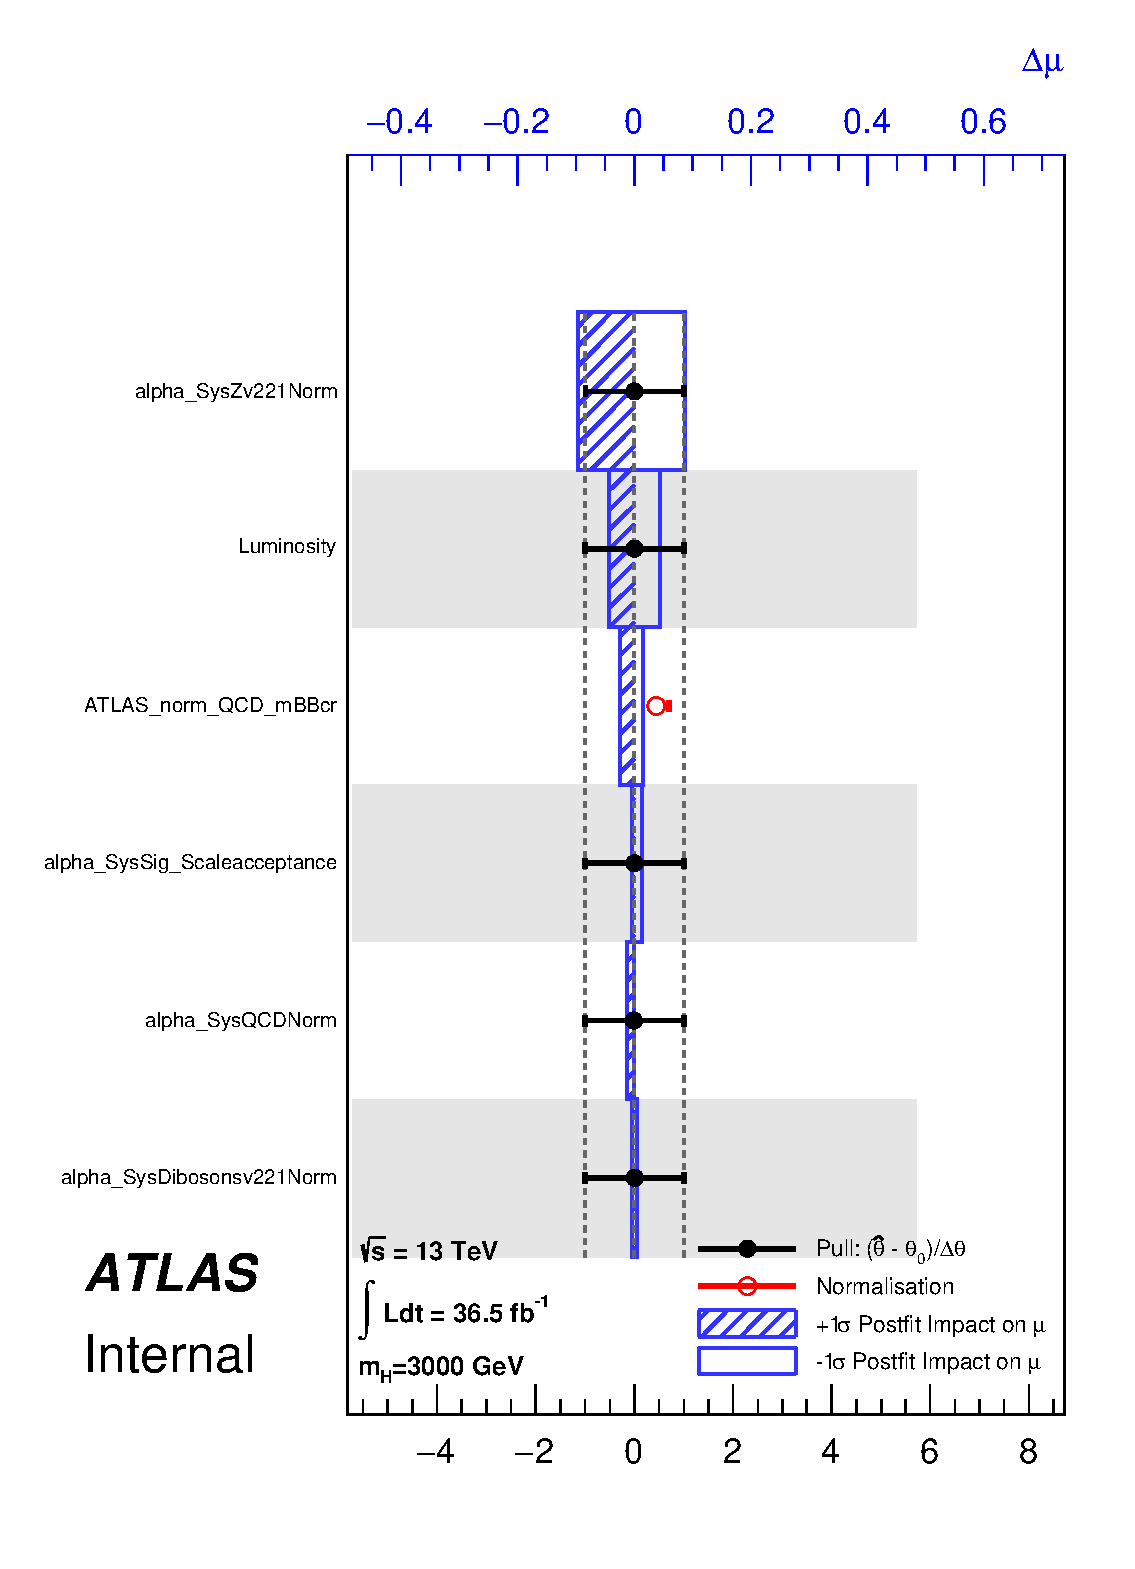
\includegraphics[width=0.45\textwidth]{chapters/dihiggs2/figures/statFit/pullPlot_X3000_mu0_unconditional.eps}
   \caption{Pull plots produced when fitting to an Asimov dataset created and profiled at $\mu=0$ for m$_X$ = 2250 and 3000~GeV for the high-mass selection. The signal strength, $\mu$, is allowed to float as a free parameter during the fit.}
  \label{fig:pullPlots2_mu_uncond}
\end{center}    
\end{figure}


\begin{figure}[!h]
\begin{center}
%\includegraphics*[width=0.60\textwidth] {chapters/dihiggs2/figures/limit_2016_TopQCDcr_NoCacc_MuQcdCr_Smooth_xSec_exp_170508_00.eps}
\includegraphics*[width=0.60\textwidth] {chapters/dihiggs2/figures/unblinded/limit_unblinded}
\caption[Expected and observed upper limits at 95\% CL on the cross-section of resonant Higgs boson pair production.]{Expected and observed upper limits at 95\% CL on the cross-section of resonant Higgs boson pair production as a function of resonant mass.}
\label{fig:finalLimit}
\end{center}
\end{figure}

\begin{figure}[!h]
\begin{center}
%\includegraphics*[width=0.60\textwidth] {chapters/dihiggs2/figures/limit_2016_TopQCDcr_NoCacc_MuQcdCr_Smooth_xSec_exp_170508_00.eps}
\includegraphics*[width=0.60\textwidth] {chapters/dihiggs2/figures/unblinded/limitSigmaDistribution}
\caption{The distribution of the observed limits compared to the expected limits. The results are consistent with a unit Gaussian expectation of zero signal (red fit). A Gaussian fit with the mean allowed to float is shown for comparison.}
\label{fig:limitSigmaDistribution}
\end{center}
\end{figure}

%\begin{figure}[hb]
%\begin{center}
%  \includegraphics[width=.75\textwidth]{figures/statFit_appendix/80009_260916-v3-observedPullPlots-x1000_HH_13TeV_260916-v3-observedPullPlots-x1000_Systs_1000_pulls_1000.png}
%  \caption{NP ranking plot for m$_X = 1000$ GeV produced when fitting to data in the control region and signal region.}
%  \label{fig:npRanking_1000}
%\end{center}    
%\end{figure}

% Future additions to the analysis that increase signal purity and/or further
% reduce the backgrounds could allow for limits to be set using a shape analysis.
  
